\documentclass[aspectratio=169,10pt]{beamer}
\usepackage[T1]{fontenc}
\usepackage[scaled=0.9]{helvet}   % stand-in for Amazon Ember (not installed)
\renewcommand{\familydefault}{\sfdefault}
\usepackage{booktabs,tabularx,multirow,makecell,colortbl,xcolor}
\usepackage{graphicx}
\usepackage{pgfplots}
\pgfplotsset{compat=1.18}
\usepackage{listings}
\usepackage{fontawesome5}

% ---- AWS template palette (dark) ----------------------------------
\definecolor{bgdark}{HTML}{161D26}
\definecolor{panel}{HTML}{232F3E}
\definecolor{awsblue}{HTML}{007DFF}
\definecolor{awspurple}{HTML}{952EFF}
\definecolor{awsmagenta}{HTML}{E433FF}
\definecolor{awsteal}{HTML}{00D6C7}
\definecolor{bodytext}{HTML}{F2F4F7}
\definecolor{inkmuted}{HTML}{A3ACB9}
\definecolor{footc}{HTML}{8B95A3}
\definecolor{rulec}{HTML}{5A6573}
\definecolor{gridc}{HTML}{333E4C}
\definecolor{vendorc}{HTML}{7B8594}
\definecolor{linkc}{HTML}{5FB0FF}
\definecolor{sectag}{HTML}{E433FF}
% extra categorical colours for charts, tuned for the dark background
\definecolor{cat1}{HTML}{EB6834}   % orange
\definecolor{cat2}{HTML}{3B8BEB}   % blue
\definecolor{cat3}{HTML}{1BAF7A}   % aqua

% footer text; override with \renewcommand{\deckfooter}{...} after \documentclass[aspectratio=169,10pt]{beamer}
\usepackage[T1]{fontenc}
\usepackage[scaled=0.9]{helvet}   % stand-in for Amazon Ember (not installed)
\renewcommand{\familydefault}{\sfdefault}
\usepackage{booktabs,tabularx,multirow,makecell,colortbl,xcolor}
\usepackage{graphicx}
\usepackage{pgfplots}
\pgfplotsset{compat=1.18}
\usepackage{listings}
\usepackage{fontawesome5}

% ---- AWS template palette (dark) ----------------------------------
\definecolor{bgdark}{HTML}{161D26}
\definecolor{panel}{HTML}{232F3E}
\definecolor{awsblue}{HTML}{007DFF}
\definecolor{awspurple}{HTML}{952EFF}
\definecolor{awsmagenta}{HTML}{E433FF}
\definecolor{awsteal}{HTML}{00D6C7}
\definecolor{bodytext}{HTML}{F2F4F7}
\definecolor{inkmuted}{HTML}{A3ACB9}
\definecolor{footc}{HTML}{8B95A3}
\definecolor{rulec}{HTML}{5A6573}
\definecolor{gridc}{HTML}{333E4C}
\definecolor{vendorc}{HTML}{7B8594}
\definecolor{linkc}{HTML}{5FB0FF}
\definecolor{sectag}{HTML}{E433FF}
% extra categorical colours for charts, tuned for the dark background
\definecolor{cat1}{HTML}{EB6834}   % orange
\definecolor{cat2}{HTML}{3B8BEB}   % blue
\definecolor{cat3}{HTML}{1BAF7A}   % aqua

% footer text; override with \renewcommand{\deckfooter}{...} after \documentclass[aspectratio=169,10pt]{beamer}
\usepackage[T1]{fontenc}
\usepackage[scaled=0.9]{helvet}   % stand-in for Amazon Ember (not installed)
\renewcommand{\familydefault}{\sfdefault}
\usepackage{booktabs,tabularx,multirow,makecell,colortbl,xcolor}
\usepackage{graphicx}
\usepackage{pgfplots}
\pgfplotsset{compat=1.18}
\usepackage{listings}
\usepackage{fontawesome5}

% ---- AWS template palette (dark) ----------------------------------
\definecolor{bgdark}{HTML}{161D26}
\definecolor{panel}{HTML}{232F3E}
\definecolor{awsblue}{HTML}{007DFF}
\definecolor{awspurple}{HTML}{952EFF}
\definecolor{awsmagenta}{HTML}{E433FF}
\definecolor{awsteal}{HTML}{00D6C7}
\definecolor{bodytext}{HTML}{F2F4F7}
\definecolor{inkmuted}{HTML}{A3ACB9}
\definecolor{footc}{HTML}{8B95A3}
\definecolor{rulec}{HTML}{5A6573}
\definecolor{gridc}{HTML}{333E4C}
\definecolor{vendorc}{HTML}{7B8594}
\definecolor{linkc}{HTML}{5FB0FF}
\definecolor{sectag}{HTML}{E433FF}
% extra categorical colours for charts, tuned for the dark background
\definecolor{cat1}{HTML}{EB6834}   % orange
\definecolor{cat2}{HTML}{3B8BEB}   % blue
\definecolor{cat3}{HTML}{1BAF7A}   % aqua

% footer text; override with \renewcommand{\deckfooter}{...} after \input{preamble}
\newcommand{\deckfooter}{\textcopyright{} \the\year, Amazon Web Services, Inc. or its affiliates.}

% ---- beamer look ---------------------------------------------------
\setbeamercolor{background canvas}{bg=bgdark}
\setbeamercolor{normal text}{fg=bodytext,bg=bgdark}
\setbeamercolor{structure}{fg=awsblue}
\setbeamercolor{frametitle}{fg=white}
\setbeamercolor{itemize item}{fg=awsteal}
\setbeamercolor{itemize subitem}{fg=inkmuted}
\setbeamercolor{enumerate item}{fg=awsteal}
\setbeamercolor{alerted text}{fg=awsmagenta}
\setbeamertemplate{navigation symbols}{}
\setbeamertemplate{itemize items}[square]
\setbeamertemplate{enumerate items}[default]
\setbeamertemplate{caption}[numbered]
\setbeamerfont{itemize/enumerate subbody}{size=\scriptsize}
\setbeamersize{text margin left=8mm,text margin right=8mm}

% section tag shown above each frame title (no divider slides)
\gdef\secname{}
\newcommand{\sect}[1]{\section{#1}\gdef\secname{#1}}
\setbeamertemplate{frametitle}{%
  \nointerlineskip\vskip3.2mm
  \ifx\secname\empty\else{\fontsize{6.5}{7}\selectfont\bfseries\color{sectag}\MakeUppercase{\secname}}\par\vskip0.9mm\fi
  {\fontsize{12.5}{14.5}\selectfont\bfseries\color{white}\insertframetitle}\par\vskip0.6mm}
\setbeamertemplate{headline}{}
\setbeamertemplate{footline}{%
  \hbox to\paperwidth{\hspace*{8mm}{\fontsize{5}{6}\selectfont\color{footc}\deckfooter}\hfill{\fontsize{6}{7}\selectfont\color{footc}\insertframenumber}\hspace*{8mm}}\vskip2.5mm}

% ---- deck macros ---------------------------------------------------
\newcommand{\hl}[1]{\textcolor{awsteal}{\textbf{#1}}}
\newcommand{\src}[1]{\vfill{\tiny\textcolor{footc}{Source: #1}}}
\newcommand{\flabel}[1]{\label{#1}\hypertarget{#1}{}}
% clickable slide references
\newcommand{\sref}[1]{\hyperlink{#1}{\textcolor{linkc}{slide~\pageref*{#1}}}}
\newcommand{\srefs}[2]{\textcolor{linkc}{slides~\hyperlink{#1}{\pageref*{#1}}--\hyperlink{#2}{\pageref*{#2}}}}
\newcommand{\plainen}[1]{\colorbox{panel}{\parbox{\dimexpr\linewidth-2\fboxsep}{\raggedright\footnotesize\textbf{In plain English:} #1}}\par\vspace{1mm}}
\newcommand{\idcard}[1]{\colorbox{panel}{\parbox{\dimexpr\textwidth-2\fboxsep}{\scriptsize #1}}}
\newcommand{\grp}[2]{\multicolumn{#1}{@{}l}{\textcolor{awsteal}{\textit{#2}}}}
\newcommand{\agi}[4]{\hyperlink{#1}{{\large\bfseries\color{awsteal}#2}\quad{\large\bfseries\color{white}#3}}\\[0.5mm]{\small\color{inkmuted}#4}\par\vspace{4mm}}
\newcommand{\bgframe}[1]{\usebackgroundtemplate{\includegraphics[width=\paperwidth,height=\paperheight]{#1}}}

\arrayrulecolor{rulec}
\lstset{basicstyle=\ttfamily\tiny\color{bodytext},breaklines=true,columns=fullflexible,
  backgroundcolor=\color{panel},frame=single,rulecolor=\color{rulec},
  keywordstyle=\color{awsteal}\bfseries,commentstyle=\color{inkmuted},showstringspaces=false}
\renewcommand{\arraystretch}{1.1}
\usetikzlibrary{arrows.meta,positioning,shapes.geometric,calc,fit,backgrounds,shadows}
\tikzset{box/.style={draw=awsblue,fill=panel,rounded corners=2pt,align=center,font=\scriptsize,inner sep=3pt,text=bodytext},
         arr/.style={-{Stealth[length=2mm]},thick,awsblue}}
\pgfplotsset{every axis/.append style={axis line style={rulec},tick style={rulec},
  tick label style={text=bodytext},label style={text=bodytext}}}

% numbered table / figure labels (one index across the deck)
\newcounter{tabno}\newcounter{figno}
\newcommand{\tabcap}[1]{\refstepcounter{tabno}{\scriptsize\bfseries\color{awsteal}Table~\thetabno\hspace{0.6em}{\color{bodytext}#1}}\par\vspace{0.2mm}}
\newcommand{\figcap}[1]{\refstepcounter{figno}{\scriptsize\bfseries\color{awsteal}Figure~\thefigno\hspace{0.6em}{\color{bodytext}#1}}\par\vspace{0.2mm}}

% ---- table helpers -------------------------------------------------
\newcommand{\tb}[1]{\texttt{#1}}
\newcolumntype{P}[1]{>{\raggedright\arraybackslash}p{#1}}
\newcolumntype{Y}{>{\raggedright\arraybackslash}X}
% substrate names in their fixed chart colours (blue / orange / aqua)
\newcommand{\smv}{\textcolor{cat2}{\textbf{microVM}}}
\newcommand{\sm}{\textcolor{cat1}{\textbf{m5}}}
\newcommand{\sg}{\textcolor{cat3}{\textbf{g6}}}

\newcommand{\deckfooter}{\textcopyright{} \the\year, Amazon Web Services, Inc. or its affiliates.}

% ---- beamer look ---------------------------------------------------
\setbeamercolor{background canvas}{bg=bgdark}
\setbeamercolor{normal text}{fg=bodytext,bg=bgdark}
\setbeamercolor{structure}{fg=awsblue}
\setbeamercolor{frametitle}{fg=white}
\setbeamercolor{itemize item}{fg=awsteal}
\setbeamercolor{itemize subitem}{fg=inkmuted}
\setbeamercolor{enumerate item}{fg=awsteal}
\setbeamercolor{alerted text}{fg=awsmagenta}
\setbeamertemplate{navigation symbols}{}
\setbeamertemplate{itemize items}[square]
\setbeamertemplate{enumerate items}[default]
\setbeamertemplate{caption}[numbered]
\setbeamerfont{itemize/enumerate subbody}{size=\scriptsize}
\setbeamersize{text margin left=8mm,text margin right=8mm}

% section tag shown above each frame title (no divider slides)
\gdef\secname{}
\newcommand{\sect}[1]{\section{#1}\gdef\secname{#1}}
\setbeamertemplate{frametitle}{%
  \nointerlineskip\vskip3.2mm
  \ifx\secname\empty\else{\fontsize{6.5}{7}\selectfont\bfseries\color{sectag}\MakeUppercase{\secname}}\par\vskip0.9mm\fi
  {\fontsize{12.5}{14.5}\selectfont\bfseries\color{white}\insertframetitle}\par\vskip0.6mm}
\setbeamertemplate{headline}{}
\setbeamertemplate{footline}{%
  \hbox to\paperwidth{\hspace*{8mm}{\fontsize{5}{6}\selectfont\color{footc}\deckfooter}\hfill{\fontsize{6}{7}\selectfont\color{footc}\insertframenumber}\hspace*{8mm}}\vskip2.5mm}

% ---- deck macros ---------------------------------------------------
\newcommand{\hl}[1]{\textcolor{awsteal}{\textbf{#1}}}
\newcommand{\src}[1]{\vfill{\tiny\textcolor{footc}{Source: #1}}}
\newcommand{\flabel}[1]{\label{#1}\hypertarget{#1}{}}
% clickable slide references
\newcommand{\sref}[1]{\hyperlink{#1}{\textcolor{linkc}{slide~\pageref*{#1}}}}
\newcommand{\srefs}[2]{\textcolor{linkc}{slides~\hyperlink{#1}{\pageref*{#1}}--\hyperlink{#2}{\pageref*{#2}}}}
\newcommand{\plainen}[1]{\colorbox{panel}{\parbox{\dimexpr\linewidth-2\fboxsep}{\raggedright\footnotesize\textbf{In plain English:} #1}}\par\vspace{1mm}}
\newcommand{\idcard}[1]{\colorbox{panel}{\parbox{\dimexpr\textwidth-2\fboxsep}{\scriptsize #1}}}
\newcommand{\grp}[2]{\multicolumn{#1}{@{}l}{\textcolor{awsteal}{\textit{#2}}}}
\newcommand{\agi}[4]{\hyperlink{#1}{{\large\bfseries\color{awsteal}#2}\quad{\large\bfseries\color{white}#3}}\\[0.5mm]{\small\color{inkmuted}#4}\par\vspace{4mm}}
\newcommand{\bgframe}[1]{\usebackgroundtemplate{\includegraphics[width=\paperwidth,height=\paperheight]{#1}}}

\arrayrulecolor{rulec}
\lstset{basicstyle=\ttfamily\tiny\color{bodytext},breaklines=true,columns=fullflexible,
  backgroundcolor=\color{panel},frame=single,rulecolor=\color{rulec},
  keywordstyle=\color{awsteal}\bfseries,commentstyle=\color{inkmuted},showstringspaces=false}
\renewcommand{\arraystretch}{1.1}
\usetikzlibrary{arrows.meta,positioning,shapes.geometric,calc,fit,backgrounds,shadows}
\tikzset{box/.style={draw=awsblue,fill=panel,rounded corners=2pt,align=center,font=\scriptsize,inner sep=3pt,text=bodytext},
         arr/.style={-{Stealth[length=2mm]},thick,awsblue}}
\pgfplotsset{every axis/.append style={axis line style={rulec},tick style={rulec},
  tick label style={text=bodytext},label style={text=bodytext}}}

% numbered table / figure labels (one index across the deck)
\newcounter{tabno}\newcounter{figno}
\newcommand{\tabcap}[1]{\refstepcounter{tabno}{\scriptsize\bfseries\color{awsteal}Table~\thetabno\hspace{0.6em}{\color{bodytext}#1}}\par\vspace{0.2mm}}
\newcommand{\figcap}[1]{\refstepcounter{figno}{\scriptsize\bfseries\color{awsteal}Figure~\thefigno\hspace{0.6em}{\color{bodytext}#1}}\par\vspace{0.2mm}}

% ---- table helpers -------------------------------------------------
\newcommand{\tb}[1]{\texttt{#1}}
\newcolumntype{P}[1]{>{\raggedright\arraybackslash}p{#1}}
\newcolumntype{Y}{>{\raggedright\arraybackslash}X}
% substrate names in their fixed chart colours (blue / orange / aqua)
\newcommand{\smv}{\textcolor{cat2}{\textbf{microVM}}}
\newcommand{\sm}{\textcolor{cat1}{\textbf{m5}}}
\newcommand{\sg}{\textcolor{cat3}{\textbf{g6}}}

\newcommand{\deckfooter}{\textcopyright{} \the\year, Amazon Web Services, Inc. or its affiliates.}

% ---- beamer look ---------------------------------------------------
\setbeamercolor{background canvas}{bg=bgdark}
\setbeamercolor{normal text}{fg=bodytext,bg=bgdark}
\setbeamercolor{structure}{fg=awsblue}
\setbeamercolor{frametitle}{fg=white}
\setbeamercolor{itemize item}{fg=awsteal}
\setbeamercolor{itemize subitem}{fg=inkmuted}
\setbeamercolor{enumerate item}{fg=awsteal}
\setbeamercolor{alerted text}{fg=awsmagenta}
\setbeamertemplate{navigation symbols}{}
\setbeamertemplate{itemize items}[square]
\setbeamertemplate{enumerate items}[default]
\setbeamertemplate{caption}[numbered]
\setbeamerfont{itemize/enumerate subbody}{size=\scriptsize}
\setbeamersize{text margin left=8mm,text margin right=8mm}

% section tag shown above each frame title (no divider slides)
\gdef\secname{}
\newcommand{\sect}[1]{\section{#1}\gdef\secname{#1}}
\setbeamertemplate{frametitle}{%
  \nointerlineskip\vskip3.2mm
  \ifx\secname\empty\else{\fontsize{6.5}{7}\selectfont\bfseries\color{sectag}\MakeUppercase{\secname}}\par\vskip0.9mm\fi
  {\fontsize{12.5}{14.5}\selectfont\bfseries\color{white}\insertframetitle}\par\vskip0.6mm}
\setbeamertemplate{headline}{}
\setbeamertemplate{footline}{%
  \hbox to\paperwidth{\hspace*{8mm}{\fontsize{5}{6}\selectfont\color{footc}\deckfooter}\hfill{\fontsize{6}{7}\selectfont\color{footc}\insertframenumber}\hspace*{8mm}}\vskip2.5mm}

% ---- deck macros ---------------------------------------------------
\newcommand{\hl}[1]{\textcolor{awsteal}{\textbf{#1}}}
\newcommand{\src}[1]{\vfill{\tiny\textcolor{footc}{Source: #1}}}
\newcommand{\flabel}[1]{\label{#1}\hypertarget{#1}{}}
% clickable slide references
\newcommand{\sref}[1]{\hyperlink{#1}{\textcolor{linkc}{slide~\pageref*{#1}}}}
\newcommand{\srefs}[2]{\textcolor{linkc}{slides~\hyperlink{#1}{\pageref*{#1}}--\hyperlink{#2}{\pageref*{#2}}}}
\newcommand{\plainen}[1]{\colorbox{panel}{\parbox{\dimexpr\linewidth-2\fboxsep}{\raggedright\footnotesize\textbf{In plain English:} #1}}\par\vspace{1mm}}
\newcommand{\idcard}[1]{\colorbox{panel}{\parbox{\dimexpr\textwidth-2\fboxsep}{\scriptsize #1}}}
\newcommand{\grp}[2]{\multicolumn{#1}{@{}l}{\textcolor{awsteal}{\textit{#2}}}}
\newcommand{\agi}[4]{\hyperlink{#1}{{\large\bfseries\color{awsteal}#2}\quad{\large\bfseries\color{white}#3}}\\[0.5mm]{\small\color{inkmuted}#4}\par\vspace{4mm}}
\newcommand{\bgframe}[1]{\usebackgroundtemplate{\includegraphics[width=\paperwidth,height=\paperheight]{#1}}}

\arrayrulecolor{rulec}
\lstset{basicstyle=\ttfamily\tiny\color{bodytext},breaklines=true,columns=fullflexible,
  backgroundcolor=\color{panel},frame=single,rulecolor=\color{rulec},
  keywordstyle=\color{awsteal}\bfseries,commentstyle=\color{inkmuted},showstringspaces=false}
\renewcommand{\arraystretch}{1.1}
\usetikzlibrary{arrows.meta,positioning,shapes.geometric,calc,fit,backgrounds,shadows}
\tikzset{box/.style={draw=awsblue,fill=panel,rounded corners=2pt,align=center,font=\scriptsize,inner sep=3pt,text=bodytext},
         arr/.style={-{Stealth[length=2mm]},thick,awsblue}}
\pgfplotsset{every axis/.append style={axis line style={rulec},tick style={rulec},
  tick label style={text=bodytext},label style={text=bodytext}}}

% numbered table / figure labels (one index across the deck)
\newcounter{tabno}\newcounter{figno}
\newcommand{\tabcap}[1]{\refstepcounter{tabno}{\scriptsize\bfseries\color{awsteal}Table~\thetabno\hspace{0.6em}{\color{bodytext}#1}}\par\vspace{0.2mm}}
\newcommand{\figcap}[1]{\refstepcounter{figno}{\scriptsize\bfseries\color{awsteal}Figure~\thefigno\hspace{0.6em}{\color{bodytext}#1}}\par\vspace{0.2mm}}

% ---- table helpers -------------------------------------------------
\newcommand{\tb}[1]{\texttt{#1}}
\newcolumntype{P}[1]{>{\raggedright\arraybackslash}p{#1}}
\newcolumntype{Y}{>{\raggedright\arraybackslash}X}
% substrate names in their fixed chart colours (blue / orange / aqua)
\newcommand{\smv}{\textcolor{cat2}{\textbf{microVM}}}
\newcommand{\sm}{\textcolor{cat1}{\textbf{m5}}}
\newcommand{\sg}{\textcolor{cat3}{\textbf{g6}}}

\renewcommand{\deckfooter}{demo\_hybrid\_terminalbench $\cdot$ agentcore-project $\cdot$ October 2026}

\title{Run full Terminal-Bench agentic RL on AWS}
\date{October 2026}

\begin{document}

%====================================================================
{\bgframe{art/bg_title.jpg}
\begin{frame}[plain]
\vspace*{4mm}
\begin{minipage}{0.60\textwidth}
{\fontsize{22}{26}\selectfont\bfseries\color{white}Run full Terminal-Bench agentic RL on AWS\par}
\vspace{3mm}
{\raggedright\large\color{white}A hybrid solution: AgentCore microVMs, m5 EC2 instances and g6 GPU Instances, plus KernelBench\par}
\vspace{8mm}
{\small\color{white}\textbf{demo\_hybrid\_terminalbench}\\slime (Qwen3-4B, fully-async GRPO) on a g6e.48xlarge trainer\par}
\vspace{3mm}
{\scriptsize\color{inkmuted}Data as of 4 October 2026 (us-west-2)}
\end{minipage}
\end{frame}}

%====================================================================
\begin{frame}
\flabel{fr:agenda}
\vspace*{1mm}
\begin{columns}[c]
\column{0.24\textwidth}
{\fontsize{24}{28}\selectfont\bfseries\color{white}Agenda}
\column{0.04\textwidth}
\tikz\fill[awsmagenta] (0,0) rectangle (0.6pt,66mm);
\column{0.70\textwidth}
\small
\agi{fr:tb}{01}{Terminal-Bench}{What it is, three tasks, one image per task, who runs where}
\agi{fr:kb}{02}{KernelBench}{GPU kernel tasks and their reward}
\agi{fr:sizes}{03}{Image sizes}{Why one sandbox product is not enough}
\agi{fr:hybrid}{04}{The hybrid solution}{Components, pipeline, sessions and instances, m5 and g6}
\agi{fr:preopen}{05}{Pre-open}{Hiding cold starts of 1 s to 2.5 min}
\agi{fr:results}{06}{Results and conclusion}{Smoke runs, training run, what is solved}
\end{columns}
\end{frame}

%====================================================================
\sect{Terminal-Bench}

\begin{frame}{Terminal-Bench: 241 real terminal tasks, each graded by its own hidden tests}
\flabel{fr:tb}
\begin{columns}[T]
\column{0.52\textwidth}
\begin{itemize}\footnotesize\setlength{\itemsep}{1.2mm}
\item \textbf{What it is:} a benchmark of tasks an agent solves \textbf{through a shell}: fix a broken
  system, configure a service, process data, attack a vulnerable app (laude-institute/terminal-bench).
\item \textbf{Each task ships:} an instruction, a \textbf{Dockerfile} (its environment), a
  \texttt{docker-compose.yaml}, and \textbf{hidden pytest tests} plus a reference solution.
\item \textbf{The reward} (RLVR, no LLM judge): after the agent stops, the tests are copied in and run;
  reward 1 if they all pass.
\item \textbf{The agent:} Qwen3-4B with \texttt{bash}, \texttt{write\_file} and \texttt{read\_file}, up to 8
  turns, running \hl{inside} the task's sandbox and calling the trainer for each turn.
\end{itemize}
\column{0.44\textwidth}
\tabcap{Corpus}
\footnotesize\setlength{\tabcolsep}{4pt}
\begin{tabular}{@{}l r@{}}
\toprule
\textbf{Tasks} & \textbf{n}\\
\midrule
single container (\texttt{client} only) & 229\\
multi-container compose (client + sidecars) & 12\\
\midrule
\textbf{total} & \hl{241}\\
\bottomrule
\end{tabular}
\vspace{2mm}
\plainen{every task is a small broken computer plus a hidden exam; the agent fixes it with shell commands and the exam scores it.}
\end{columns}
\src{terminalbench/tasks/manifest.json (fetch\_terminalbench.py, laude-institute/terminal-bench main), checked 4 Oct 2026.}
\end{frame}

%====================================================================
\begin{frame}{Three tasks show why each needs its own environment and substrate}
\flabel{fr:tbex}
\tabcap{Example tasks}
\scriptsize\setlength{\tabcolsep}{3pt}
\begin{tabular}{@{}p{0.17\textwidth} p{0.47\textwidth} p{0.30\textwidth}@{}}
\toprule
\textbf{Task} & \textbf{Instruction (abridged)} & \textbf{Environment $\rightarrow$ substrate}\\
\midrule
\textbf{jq-data-processing}\newline\textcolor{inkmuted}{easy, data processing} &
``Use jq to transform \texttt{/app/users.json}: keep active users, reformat the ISO-8601 last\_login
dates, write \texttt{/app/active\_users\_report.json}.'' &
One container, small image (jq + data file).\newline\textcolor{awsblue}{\textbf{AgentCore microVM}}\\[1mm]
\textbf{postgres-csv-clean}\newline\textcolor{inkmuted}{medium, file operations} &
``Connect to the Postgres DB from the compose config, import \texttt{customers.csv}, clean the data,
export a cleaned CSV.'' &
\textbf{Two containers}: \texttt{client} + a \texttt{postgres:16} sidecar on a private network.\newline
\textcolor{cat1}{\textbf{m5 EC2}} (compose project)\\[1mm]
\textbf{mteb-eval}\newline\textcolor{inkmuted}{medium, data science} &
``Evaluate an embedding model from Hugging Face on STS12 with \texttt{mteb} so that cosine\_spearman
$>$ 0.7; store the model in the default cache.'' &
One container, but a \textbf{6.7\,GB} image (torch + models): over the 2\,GB microVM cap.\newline
\textcolor{cat1}{\textbf{m5 EC2}}\\
\bottomrule
\end{tabular}
\par\vspace{2mm}
\plainen{the environment decides the substrate: small and single-container goes to a microVM; several containers, x86-only or a big image goes to an m5.}
\src{\tb{terminalbench/tasks/manifest.json}, \tb{images.csv}, \tb{route\_by\_image.json}; checked 4 Oct 2026.}
\end{frame}

%====================================================================
\begin{frame}{The route is data: 241 tasks $\rightarrow$ 236 routed $\rightarrow$ 193 with a trusted reward}
\flabel{fr:route}
\begin{columns}[T]
\column{0.50\textwidth}
\tabcap{Where each task goes and why}
\scriptsize\setlength{\tabcolsep}{3pt}
\begin{tabularx}{\linewidth}{@{}Y r@{}}
\toprule
\textbf{Step} & \textbf{Tasks}\\
\midrule
Corpus (229 single + 12 compose) & 241\\
\smv: arm64 build ships ($\le$ 2\,GB) & 218\\
\quad build failed / over 2\,GB & 7 / 4\\
\sm: compose, x86-only, $>$ 2\,GB, or microVM oracle failed & 78\\
\quad built on the m5 builder & 71\\
\midrule
\textbf{Routed} (\smv{} / \sm) & 165 / 71\\
\textbf{Oracle passes} (\smv{} / \sm) & \hl{163 / 30 = 193}\\
\bottomrule
\end{tabularx}
\column{0.46\textwidth}
\begin{itemize}\scriptsize\setlength{\itemsep}{1mm}
\item \textbf{Every route comes from a measured result}: build status and size (\tb{images.csv}),
  compose or not (\tb{manifest.json}), and the reference solution run on the substrate (\tb{oracle.csv}).
\item \textbf{A task that fails its oracle on a microVM is retried on the m5}, which gives it root, raw
  networking and x86; it is kept where it passes.
\item \tb{image\_routing.py} \textbf{refuses an unmapped task}: no silent fallback to the wrong sandbox.
\item \textbf{193 usable vs 165} for the microVM-only demo (\tb{demo\_cpu\_terminalbench}): 17\,\% more of the corpus.
\item \textbf{Not rescued:} 7 m5 builds fail upstream (e.g. \tb{fix-git}: its GitHub repo was deleted;
  \tb{leelachess0}: file 404).
\end{itemize}
\end{columns}
\src{\tb{make\_figures.py} $\rightarrow$ \tb{data.json} (corpus block), from \tb{terminalbench/tasks/\{manifest.json, images.csv, images\_docker.csv, oracle.csv, route\_by\_image.json\}}; checked 4 Oct 2026.}
\end{frame}

%====================================================================
\sect{KernelBench}

\begin{frame}{KernelBench: write a faster CUDA kernel, graded on a real GPU}
\flabel{fr:kb}
\begin{columns}[T]
\column{0.52\textwidth}
\begin{itemize}\footnotesize\setlength{\itemsep}{1.2mm}
\item \textbf{The task:} given a reference PyTorch \tb{Model}, write \tb{ModelNew} in \tb{solution.py}: same
  outputs (atol/rtol $10^{-2}$), on CUDA, ideally faster (custom kernels, fusion, better ops).
\item \textbf{Rows:} 40 level-1 tasks (single ops) for training, 10 level-2 tasks (fused ops) held out.
  They are \textbf{mixed into the same batch} as Terminal-Bench rows.
\item \textbf{The sandbox:} one \hl{AgentCore g6 Instance} (g6.xlarge, NVIDIA L4) per episode, from the
  capacity provider \tb{acs\_tbh\_gpu\_cp}. No Terminal-Bench task needs a GPU.
\item \textbf{The checker} (hidden, random name, nonce'd \tb{PASSED} line) builds \tb{ModelNew} next to
  \tb{Model}, checks shape, values and device, and prints \tb{speedup=}.
\end{itemize}
\column{0.44\textwidth}
\tabcap{Reward (\tb{TB\_KB\_SPEEDUP\_MIN} = 1.10)}
\footnotesize\setlength{\tabcolsep}{4pt}
\begin{tabular}{@{}l r@{}}
\toprule
\textbf{Outcome} & \textbf{Reward}\\
\midrule
correct and $\ge$ 1.10$\times$ faster & \hl{1.0}\\
correct, not faster & 0.5\\
wrong, crashed or not on CUDA & 0\\
\bottomrule
\end{tabular}
\par\vspace{2mm}
\begin{itemize}\scriptsize\setlength{\itemsep}{0.6mm}
\item The first reward was correctness only: copying \tb{Model} onto CUDA scored 1, so groups
  were all 1s (smoke 4: 48 of 75).
\item Copies of the reference measure 1.00--1.03$\times$, so the 1.10$\times$ bar is above timing noise.
\end{itemize}
\end{columns}
\src{\tb{kernelbench/}, \tb{data/kernelbench\_\{train,eval\}.jsonl}, \tb{deploy/Dockerfile.kernelbench\_gpu}, demo README (KernelBench on the g6 tier); checked 4 Oct 2026.}
\end{frame}

%====================================================================
\sect{Image sizes}

\begin{frame}{Image sizes: most tasks fit a microVM, the tail and the GPU task do not}
\flabel{fr:sizes}
\figcap{Task image sizes against the 2\,GB microVM image cap}
\centering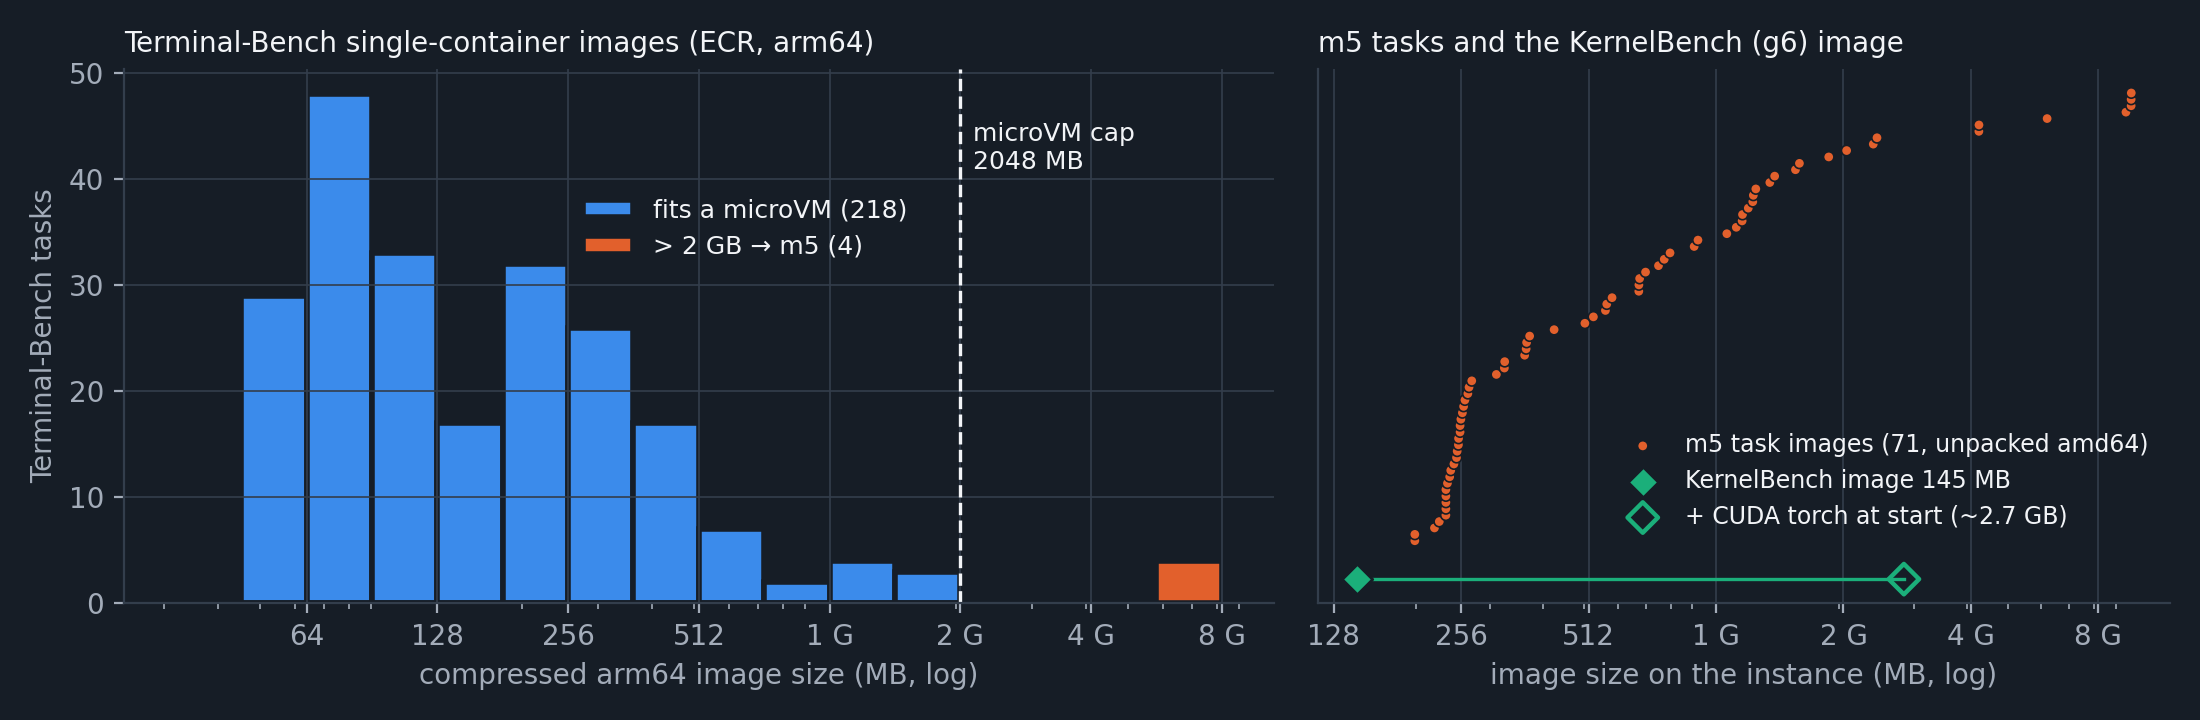
\includegraphics[width=0.94\textwidth]{fig_image_sizes.png}\par
\raggedright\vspace{1mm}
\begin{columns}[T]
\column{0.48\textwidth}
\begin{itemize}\scriptsize\setlength{\itemsep}{0.5mm}
\item \textbf{arm64 microVM images:} p50 \textbf{127\,MB}, p95 620\,MB, largest that fits 2.0\,GB.
\item \textbf{4 tasks are 6.5--6.7\,GB} (\tb{mteb-*}, \tb{png-generation}): no microVM can take them.
\end{itemize}
\column{0.48\textwidth}
\begin{itemize}\scriptsize\setlength{\itemsep}{0.5mm}
\item \textbf{m5 images} (unpacked, amd64): p50 525\,MB, up to 9.8\,GB; the m5 has a 40\,GB disk.
\item \textbf{KernelBench:} the 2\,GB cap also applies to capacity-provider Runtimes, so the image is
  145\,MB and installs CUDA torch ($\sim$2.7\,GB) at container start ($\sim$90\,s).
\end{itemize}
\end{columns}
\src{\tb{images.csv} (ECR compressed size), \tb{images\_docker.csv} (\tb{docker image inspect}); \tb{make\_figures.py}; checked 4 Oct 2026.}
\end{frame}

%====================================================================
\sect{The hybrid solution}

\begin{frame}{The demo: use case covered, why this demo, design considerations}
\flabel{fr:hybrid}
\scriptsize\setlength{\tabcolsep}{4pt}
\tabcap{The demo in three answers}
\begin{tabularx}{\textwidth}{@{}P{0.17\textwidth}Y@{}}
\toprule
\textbf{Use case covered} & Agentic RL on a benchmark whose environments \textbf{do not all fit one sandbox product}: most
tasks are one small container, but some need several networked containers, an x86 CPU, a multi-GB image,
root powers a capability-less microVM does not grant, or a \textbf{GPU} (KernelBench).\\
\textbf{Why this demo} & It trains on \hl{the whole usable corpus} (193 Terminal-Bench tasks + 50 KernelBench) instead of
the 165 the microVM pool alone can validate. It shows the sandbox tier can be \textbf{heterogeneous without
touching the RL side}: agent loop, grader, reward, pre-open and metrics are one code path for all three
substrates. \tb{eval/terminalbench} stays the same held-out set as \tb{demo\_cpu\_terminalbench}.\\
\textbf{Design considerations} & \textbf{One protocol, three transports:} every image is the task's own Dockerfile plus the same
wrapper (standalone \tb{/opt/acs/py} + stdlib \tb{acs\_http\_server.py}); AgentCore invokes it on a microVM or g6,
the trainer POSTs to it on an m5 (\tb{DockerComposeSandbox} only swaps the transport)
\textperiodcentered{} \textbf{routing is data}, not a hand-kept list (\sref{fr:route})
\textperiodcentered{} \textbf{one session per sandbox}: a fresh microVM, a warm m5 reused only after a
\textbf{verified} reset, a fresh g6 Instance
\textperiodcentered{} \textbf{per-episode compose rewrite}: fixed container names, host ports and \tb{./} mounts
made unique, privileged/host-network/\tb{docker.sock} refused
\textperiodcentered{} \textbf{hidden tests stay hidden}: task dirs reach the m5 without \tb{tests/} or the solution
\textperiodcentered{} \textbf{rejected:} running compose on AgentCore (no capabilities, no Docker daemon), the g6e as
Docker host (it trains), g5 for KernelBench (accepted, but g6 is cheaper: \$0.80 vs \$1.01/h).\\
\bottomrule
\end{tabularx}
\src{\tb{code/demos/demo\_hybrid\_terminalbench/README.md}; \tb{docs/terminalbench-hybrid-demo-plan.md}; checked 4 Oct 2026.}
\end{frame}

%====================================================================
\begin{frame}{One trainer, one router, three sandbox substrates}
\flabel{fr:arch}
\figcap{Components: the trainer routes each row; the agent loop runs inside the sandbox and dials back}
\centering
\begin{tikzpicture}[node distance=4mm]
\node[box,minimum width=44mm,minimum height=30mm,align=left] (tr) {%
  \textbf{\small g6e.48xlarge trainer} (8$\times$L40S)\\[1mm]
  slime fully-async GRPO, Qwen3-4B\\
  4 GPUs train $\cdot$ 4 GPUs SGLang\\
  \tb{AnthropicAdapter} per engine\\[1mm]
  \textbf{\tb{TerminalBenchPool}}\\
  route map $\cdot$ pre-open $\cdot$ gates\\
  grader (hidden tests)};
\node[box,draw=cat2,right=26mm of tr,yshift=13mm,text width=54mm,align=left] (mv) {%
  \textbf{\textcolor{cat2}{AgentCore microVM}}\quad 218 Runtimes \tb{acs\_tbh\_*}\\
  arm64, $\le$ 2\,GB $\cdot$ 1 session = 1 microVM};
\node[box,draw=cat1,right=26mm of tr,text width=54mm,align=left] (m5) {%
  \textbf{\textcolor{cat1}{m5 EC2}}\quad warm pool, $\le$ 24 \tb{m5.xlarge}\\
  Docker + compose agent $\cdot$ 1 session = 1 VM};
\node[box,draw=cat3,right=26mm of tr,yshift=-13mm,text width=54mm,align=left] (g6) {%
  \textbf{\textcolor{cat3}{AgentCore g6 Instance}}\quad \tb{acs\_tbhgpu\_kernelbench}\\
  g6.xlarge L4 $\cdot$ 1 session = 1 instance};
\draw[arr,cat2] (tr.east)+(0,4mm) -- node[above,sloped,font=\tiny,text=inkmuted]{InvokeAgentRuntime} (mv.west);
\draw[arr,cat1] (tr.east) -- node[above,font=\tiny,text=inkmuted]{EC2 API + HTTP} (m5.west);
\draw[arr,cat3] (tr.east)+(0,-4mm) -- node[below,sloped,font=\tiny,text=inkmuted]{InvokeAgentRuntime} (g6.west);
\node[font=\tiny,text=inkmuted,align=left,right=2mm of m5] {agent loop runs\\here and calls\\\tb{/v1/messages}\\back over the VPC};
\end{tikzpicture}
\par\vspace{2mm}\raggedright
\begin{columns}[T]
\column{0.32\textwidth}
\scriptsize\textbf{\textcolor{cat2}{microVM}:} 163 tasks. Managed by AgentCore; an idle session is wiped after 15\,min, so a heartbeat keeps pre-opened ones alive.
\column{0.32\textwidth}
\scriptsize\textbf{\textcolor{cat1}{m5}:} 30 tasks. \textbf{Our code} launches and terminates them (boto3, the g6e's role), from a baked AMI; images from ECR.
\column{0.32\textwidth}
\scriptsize\textbf{\textcolor{cat3}{g6}:} KernelBench. In an AgentCore-managed account: \textbf{not in our EC2 console}; one CloudWatch log stream per session.
\end{columns}
\src{\tb{agentcore\_slime\_demo/\{terminalbench\_pool, docker\_compose\_sandbox, ec2\_episode\_sandbox\}.py}, \tb{image\_routing.py}, \tb{run.sh}; checked 4 Oct 2026.}
\end{frame}

%====================================================================
\begin{frame}{One episode is the same five steps on every substrate}
\flabel{fr:pipeline}
\tabcap{What \tb{TerminalBenchPool} does per episode, by substrate}
\scriptsize\setlength{\tabcolsep}{3pt}
\begin{tabularx}{\textwidth}{@{}P{0.13\textwidth}YYY@{}}
\toprule
\textbf{Step} & \textbf{\textcolor{cat2}{microVM}} & \textbf{\textcolor{cat1}{m5 EC2 (warm)}} & \textbf{\textcolor{cat3}{g6 Instance}}\\
\midrule
1. Route & \tb{arn:\ldots/acs\_tbh\_<task>} & \tb{docker://<ip>:18300/<task>} & \tb{gpu:arn:\ldots/}\newline\tb{acs\_tbhgpu\_kernelbench}\\
2. Open (ahead) & new \tb{runtimeSessionId}; first invoke boots the microVM & idle VM (prefer one holding the images) or \tb{run\_instances}; ECR pull; \tb{compose up} & new session id; first invoke launches a g6, then torch install\\
3. Agent loop & \multicolumn{3}{>{\centering\arraybackslash}X}{mini\_claude (\tb{bash} / \tb{write\_file} / \tb{read\_file}), up to 8 turns $\times$ 1024 tokens, \textbf{inside the sandbox}, calling the trainer's adapter}\\
4. Grade & inject \tb{tests/}, run pytest & same, in the client & hidden checker: correctness + \tb{speedup=}\\
5. Close & \tb{StopRuntimeSession} & \tb{compose down -v} + \tb{reset\_check}; clean $\rightarrow$ pool, dirty $\rightarrow$ terminate & \tb{StopRuntimeSession} (instance released)\\
\midrule
Open cost (smoke 6, p50) & \textbf{2\,s} & \textbf{68\,s} (cold launch 34--51\,s + pull) & \textbf{135\,s} (boot + $\sim$90\,s torch)\\
Episode p50 & 24\,s (agent 12\,s, grade 9\,s) & 69\,s (agent 14\,s, grade 7\,s) & --\\
\bottomrule
\end{tabularx}
\par\vspace{1mm}
\plainen{the RL code never asks which substrate it is on; only the open cost differs (2\,s to over 2\,min).}
\src{\tb{logs/smoke6-hybrid\_*.log} (\tb{[demo]} \tb{agent\_ms}, \tb{grade\_ms}, \tb{episode\_ms}, \tb{open\_ms}); m5 per-episode probe; checked 4 Oct 2026.}
\end{frame}

%====================================================================
\begin{frame}{Sessions and instances: one session per instance, three lifecycles}
\flabel{fr:sessions}
\begin{columns}[T]
\column{0.54\textwidth}
\tabcap{Who owns each instance, and how it ends}
\scriptsize\setlength{\tabcolsep}{3pt}
\begin{tabularx}{\linewidth}{@{}P{0.20\linewidth}YYY@{}}
\toprule
& \textbf{\textcolor{cat2}{microVM}} & \textbf{\textcolor{cat1}{m5}} & \textbf{\textcolor{cat3}{g6}}\\
\midrule
Managed by & AgentCore & \textbf{our trainer} & AgentCore\\
Reused? & no, fresh & yes, after a verified reset & no, fresh\\
Isolation & own kernel & own VM per session & own instance\\
Visible in & CloudWatch & our EC2 console & CloudWatch only\\
Ends by & stop / 15-min idle & 5 ways (right) & stop / 600\,s idle\\
\bottomrule
\end{tabularx}
\par\vspace{2mm}
\tabcap{Warm m5 pool in smoke 6}
\scriptsize
\begin{tabular}{@{}l r@{}}
\toprule
instances launched / episodes on a reused one & 24 / 10\\
pool peak (cap \tb{TB\_M5\_MAX\_INSTANCES}) & 24 (24)\\
dirty resets / retired & \hl{0 / 0}\\
\bottomrule
\end{tabular}
\column{0.42\textwidth}
\begin{itemize}\scriptsize\setlength{\itemsep}{0.8mm}
\item \textbf{Verified reset} after every m5 episode: no containers, volumes or extra networks, empty episode
  dir, $\ge$ 8\,GB disk. Dirty or unhealthy $\rightarrow$ terminated, never reused. No periodic recycle.
\item \textbf{m5 termination, 5 ways:} trainer \tb{atexit}; \tb{5\_run.sh} \tb{gc-episodes}; next pool start;
  \tb{6\_cleanup.sh}; a \textbf{dead-man switch} (no trainer call for 30\,min $\rightarrow$ the VM shuts
  itself down = terminate).
\item \textbf{m5 hardening:} no IAM role; IMDSv2 hop 1 and blocked from containers; containers cannot
  reach the host; agent API needs a secret and the trainer's SG.
\item \textbf{g6:} a launch per session, so a pre-open must start $\sim$2.5\,min early (\sref{fr:preopen}).
\end{itemize}
\end{columns}
\src{\tb{agentcore\_slime\_demo/ec2\_episode\_sandbox.py} (\tb{WarmPool}), \tb{m5\_agent/bootstrap.sh}; \tb{logs/smoke6-hybrid\_*.log} (\tb{warm\_reused}, \tb{warm\_instances}); checked 4 Oct 2026.}
\end{frame}

%====================================================================
\sect{Pre-open}

\begin{frame}{Pre-open hides cold starts from 2\,s to 2.5\,min behind the running batch}
\flabel{fr:preopen}
\figcap{Median wait for the sandbox at episode start: measured with pre-open vs the open time it hides}
\centering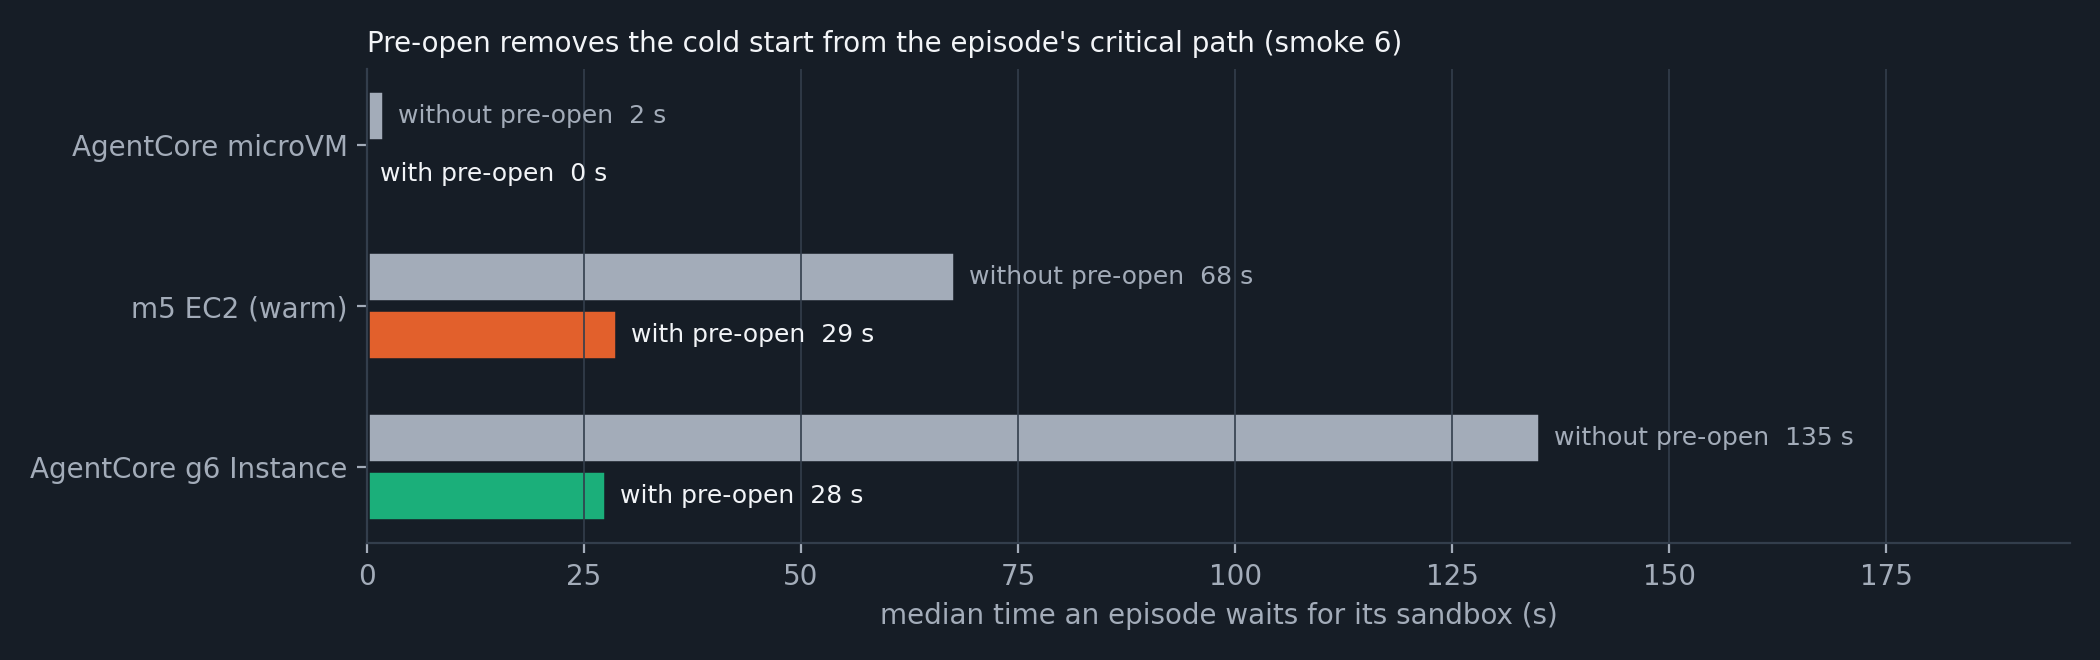
\includegraphics[width=0.84\textwidth]{fig_preopen.png}\par
\raggedright\vspace{1mm}
\begin{columns}[T]
\column{0.50\textwidth}
\tabcap{Smoke 6, by substrate}
\tiny\setlength{\tabcolsep}{3pt}
\begin{tabularx}{\linewidth}{@{}Y r r r r@{}}
\toprule
& \textbf{n} & \textbf{no wait} & \textbf{wait p90} & \textbf{saved}\\
\midrule
\textcolor{cat2}{microVM} (2 batches ahead) & 177 & 121 & 5.6\,s & 4\,min\\
\textcolor{cat1}{m5} (5 batches ahead) & 34 & 16 & 61\,s & 23\,min\\
\textcolor{cat3}{g6} (5 batches ahead) & 52 & 22 & 100\,s & \hl{80\,min}\\
\bottomrule
\end{tabularx}
\column{0.46\textwidth}
\tabcap{g6 session cap vs start wait}
\tiny\setlength{\tabcolsep}{3pt}
\begin{tabular}{@{}l r r r@{}}
\toprule
\textbf{Run} & \textbf{cap} & \textbf{wait p50} & \textbf{no wait}\\
\midrule
smoke 4 & 8 & 240\,s & 0 / 76\\
smoke 5 & 16 & 82\,s & 5 / 36\\
smoke 6 & 32 & \hl{28\,s} & 22 / 52\\
\bottomrule
\end{tabular}
\par\vspace{0.5mm}{\tiny A cap of 8 equals one group, so nothing could open ahead.}
\end{columns}
\src{\tb{logs/smoke\{4mix,5,6\}-hybrid\_*.log} (\tb{[demo]} \tb{open\_wait\_ms}, \tb{open\_ms}); ``saved'' = $\sum$ max(0, open $-$ wait); \tb{make\_figures.py}; checked 4 Oct 2026.}
\end{frame}

%====================================================================
\sect{Results and conclusion}

\begin{frame}{Five smoke runs: the pipeline works on all three substrates}
\flabel{fr:results}
\tabcap{Smoke runs on 4 Oct 2026 (train + eval episodes; solved / episodes; infra errors)}
\scriptsize\setlength{\tabcolsep}{3pt}
\begin{tabularx}{\textwidth}{@{}P{0.12\textwidth}P{0.15\textwidth}P{0.15\textwidth}P{0.14\textwidth}Y@{}}
\toprule
\textbf{Run} & \textbf{\textcolor{cat2}{microVM}} & \textbf{\textcolor{cat1}{m5}} & \textbf{\textcolor{cat3}{g6 KernelBench}} & \textbf{Eval and change}\\
\midrule
smoke 2 & 17 / 401; 1 err & 0 / 88; 0 & -- & TB 2/62; final ckpt save hung $\rightarrow$ fixed\\
smoke 3 & 16 / 382; \hl{0} & 0 / 88; \hl{0} & -- & \textbf{passed}; TB 4/62, m5 0/8\\
smoke 4 (mix) & 13 / 322; 1 & 0 / 58; 1 & 48 / 75; 0 & \textbf{passed}; KB 16/20 $\rightarrow$ reward too easy\\
smoke 5 & 6 / 157; 0 & 0 / 34; 0 & 26$\times$0.5; 0 & \textbf{passed}; speedup-gated reward, g6 cap 16\\
smoke 6 & 4 / 177; 1 & 0 / 34; 0 & 8$\times$1, 34$\times$0.5; 0 & \textbf{passed}; KB mean 0.45, up to 1.38$\times$; cap 32\\
\bottomrule
\end{tabularx}
\par\vspace{2mm}
\begin{columns}[T]
\column{0.48\textwidth}
\begin{itemize}\scriptsize\setlength{\itemsep}{0.8mm}
\item \textbf{Infra is solved:} 4 infra errors in $\sim$1{,}900 episodes over 5 runs, all three substrates.
\item \textbf{KernelBench gives a gradient:} with the gated reward, groups mix 0, 0.5 and 1.
\end{itemize}
\column{0.48\textwidth}
\begin{itemize}\scriptsize\setlength{\itemsep}{0.8mm}
\item \textbf{The m5 tasks are hard:} 0 solved in 302 episodes. They are the compose, x86 and big-image tail.
\item \textbf{Terminal-Bench eval} on the microVM set: 1--4 of 62, as in \tb{demo\_cpu\_terminalbench}.
\end{itemize}
\end{columns}
\src{\tb{logs/smoke\{2,3,4mix,5,6\}-hybrid\_*.\{log,eval.csv\}}; \tb{make\_figures.py} $\rightarrow$ \tb{data.json} (runs); checked 4 Oct 2026.}
\end{frame}

%====================================================================
\begin{frame}{The 48-step training run is in progress}
\flabel{fr:train}
\begin{columns}[T]
\column{0.50\textwidth}
\tabcap{\tb{train48}, started 4 Oct 2026 15:24 UTC (status at 16:24)}
\scriptsize\setlength{\tabcolsep}{3pt}
\begin{tabularx}{\linewidth}{@{}Y r@{}}
\toprule
steps done & 19 of 48\\
mean step time & 130\,s\\
episodes / solved & 935 / 108\\
infra errors & \hl{1}\\
expected end & $\approx$ 17:50 UTC + eval\\
\bottomrule
\end{tabularx}
\column{0.46\textwidth}
\tabcap{Train reward per step (\tb{rollout/raw\_reward})}
\scriptsize
steps 0--9:\quad 0, 0, .25, .25, 0, .13, .11, 0, .02, 0\\[0.5mm]
steps 10--18:\quad .08, 0, 0, .22, 0, .13, 0, .13, 0
\par\vspace{2mm}
\begin{itemize}\scriptsize\setlength{\itemsep}{0.6mm}
\item Noisy and flat so far, as expected at this point.
\item Final rewards and eval go here when the run ends.
\end{itemize}
\end{columns}
\src{\tb{logs/train48-hybrid\_20261004\_152433.log}; snapshot 4 Oct 2026 16:24 UTC.}
\end{frame}

%====================================================================
\begin{frame}{Conclusion: every task gets a sandbox it runs on; the reward is what is left}
\flabel{fr:concl}
\tabcap{What the demo shows}
\scriptsize\setlength{\tabcolsep}{4pt}
\begin{tabularx}{\textwidth}{@{}P{0.03\textwidth}P{0.3\textwidth}Y P{0.09\textwidth}@{}}
\toprule
& \textbf{Conclusion} & \textbf{Evidence} & \textbf{Slides}\\
\midrule
1 & \textbf{A hybrid tier covers the corpus} & 193 usable Terminal-Bench tasks vs 165 on microVMs alone, plus KernelBench on g6 & \srefs{fr:route}{fr:sizes}\\
2 & \textbf{The RL side does not change} & one agent loop, grader, pre-open and metrics path for microVM, m5 and g6 & \srefs{fr:arch}{fr:pipeline}\\
3 & \textbf{Infra is reliable} & 4 infra errors in $\sim$1{,}900 smoke episodes; 0 dirty warm resets & \srefs{fr:sessions}{fr:results}\\
4 & \textbf{Pre-open depth must match boot time} & g6 start wait p50 240\,s $\rightarrow$ 28\,s with cap 32 and 5 batches ahead & \sref{fr:preopen}\\
5 & \textbf{The reward limits learning} & TB eval 1--4 of 62; 0 of 302 m5 episodes solved; KB needed a speedup gate & \sref{fr:results}\\
\bottomrule
\end{tabularx}
\par\vspace{1.5mm}
\tabcap{Next steps}
\scriptsize
\begin{tabularx}{\textwidth}{@{}P{0.03\textwidth}P{0.4\textwidth}Y@{}}
\toprule
1 & Finish the 48-step run & running (\sref{fr:train})\\
2 & Partial credit from \tb{tests\_passed} / \tb{tests\_total} & more GRPO groups with a gradient, esp.\ on m5 tasks\\
3 & Host the CUDA torch wheel in S3 & cut the g6 open from $\sim$2.5\,min\\
4 & Stop the m5 builder when not building & it is not needed for training\\
\bottomrule
\end{tabularx}
\src{This deck; checked 4 Oct 2026.}
\end{frame}

%====================================================================
{\bgframe{art/bg_close.png}
\begin{frame}[plain]
\vfill
{\fontsize{22}{26}\selectfont\bfseries\color{white}Thank you\par}
\vspace{3mm}
{\small\color{inkmuted}\tb{code/demos/demo\_hybrid\_terminalbench}\par}
\vfill
\end{frame}}

\end{document}
